%f='selfrep'; b='selfrep'; pdflatex $f.tex && bibtex $f && pdflatex $f.tex && pdflatex $f.tex && rm $f.log $f.aux && evince $f.pdf &>/dev/null &disown



\documentclass[12pt]{article}
\usepackage[margin=1in]{geometry}
\usepackage[protrusion=true,
            expansion=true]{microtype}
%\usepackage{amssymb}
%\usepackage{amsmath}
\usepackage{booktabs}
\usepackage{color}
\usepackage[usenames,
            dvipsnames]{xcolor}
\usepackage{graphicx}
\usepackage{caption}
\usepackage{subcaption}

\usepackage{kpfonts}
\usepackage[T1]{fontenc}
\usepackage{setspace}
\singlespacing
%\onehalfspacing
%\doublespacing

\newcommand{\term}[1]{\emph{#1}}

\begin{document}

\title{Programs that Program}

\author{Keenan Breik, Jason Liang}
\date{}
\maketitle

\begin{abstract}
Evolutionary computation allows computers to automatically solve problems that can be cast as optimization problems. Until now, instantiations have been hand designed. We propose to allow computers to automatically design such instantiations by using evolutionary computation itself. To do so, we desire programs that write other programs and thereby explore a search space. In this paper, we demonstrate that neural networks (which can behave as programs or program components) can generate other meaningful neural networks.
\end{abstract}

\section*{Introduction}
%todo: write an introduction that elaborates on the abstract.

The following is a quick overview of the rest of the paper: In section \ref{feedforward}, we will go over methods for constructing self-replicating feed-forward neural networks. Next, in section \ref{results}, we will discuss experimental results. Finally in the last section, we present conclusions and future work.

\section{Self-Replicating Feed-forward Neural Networks} \label{feedforward}

To create a self-replicating feed-forward neural network, we first use the pyBrain neural network library \cite{schaul2010} to create an initial neural network that has a fixed topology. By fixed topology, we mean that the number of input neurons, output neurons, hidden layers, neurons, and number of connections remain constant. The only parameters we plan to optimize in order to generate self-replicating neural networks are  the weights of the connections between neurons. Since a feed-forward neural network can have many variations in its topology, we have chosen a simple structure that makes the most sense. 

One major challenge is deciding what kind of input to feed into the neural network and how to interpret the output of the neural network as another neural net. For simplicity, we decided on giving our neural network a N-bit vector of binary numbers as input. If we topologically linearize all the connections in the neural network, we can associate the value of binary vector with a corresponding connection. For example, the binary vector 1001 can be associated with the 5th connection in a small network with 8 connections in total. Accordingly, the output of the neural network is a single value and it represents the weight of the connection specified by the input vector. Thus, by feeding the neural network a set of inputs that map to all the connections in the network, we can generate weights for each of connections. This means that the network is capable of generating another net exactly like itself in topology, but with possibly different connection weights. 

The next step is come up with a method to optimize the connection weights of the original network such that child network generated also has the same connection weight. Given the lack of gradients in this problem, we decide to rely on a black-box optimization approach to optimize the connection weights of the parent network. Thus we will require a fitness function that evaluates how close the the neural network is to generating a child network exactly like itself. To compute a fitness value, as seen in Fig.~\ref{pseudo}, we use the parent network to compute the connection weights of the child network, determine the error between the new connection weight and its original value in the parent network, and return the sum of all the errors. Now we can try a variety of different black-box optimization methods, including genetic algorithms \cite{deb2002fast}, CMAES \cite{hansen2003reducing}, and NES \cite{wierstra2008natural} to try to minimize the error and maximize the fitness of the neural network. Experimentally, we found that using CMAES resulted the most improvement in fitness every generation. 

\begin{figure}[h]
\begin{center}
  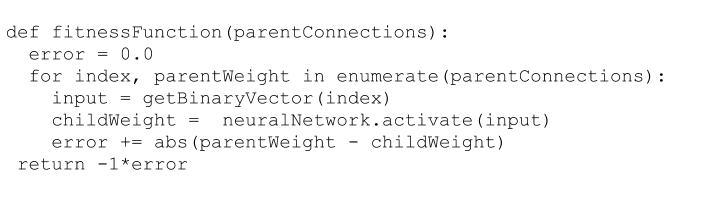
\includegraphics[width=0.8\linewidth]{pseudo.png}
\end{center}
   \caption{Function for computing fitness of a neural network. For each connection in the parent network, we convert it into a binary vector, feed it as input, and get the connection weight of the same connection in the child network. We compare the difference between the child and parent weights and sum up all differences as error, which is then inverted to become a fitness value.}
\label{pseudo}
\end{figure} 

\section{Experimental Results} \label{results}

\bibliography{selfrep}
\bibliographystyle{plain}

\end{document}
